\documentclass[10pt, compress]{beamer}

\usetheme{m}
\usepackage{soul}
\usepackage{natbib}
\bibliographystyle{unsrt}
\usepackage{booktabs}
\usepackage[scale=2]{ccicons}
\usepackage{minted}
\usepackage{graphicx}
\usepackage{wrapfig}
\usepackage{listings}
\usepackage{xcolor}
\usepackage{minted}
\usepackage{amsmath}
\usepackage{enumitem}
\usepackage{float}
\usepackage{tikz}
\usepackage{standalone}
\usepackage{algorithm}
\usepackage{algorithmicx}
\usepackage[noend]{algpseudocode}
\usemintedstyle{trac}
\renewcommand\algorithmicdo{}
\renewcommand\algorithmicthen{}
\newcolumntype{C}[1]{>{\centering\let\newline\\\arraybackslash\hspace{0pt}}m{#1}}

\lstdefinestyle{asm}{
belowcaptionskip=1\baselineskip,
keepspaces,
breaklines=true,
tabsize=8,
frame=L,
xleftmargin=\parindent,
language=[x86masm]Assembler,
showstringspaces=false,
basicstyle=\footnotesize\ttfamily,
keywordstyle=\bfseries\color{green!40!black},
commentstyle=\itshape\color{purple!40!black},
identifierstyle=\color{blue},
stringstyle=\color{orange},
columns=fullflexible,
}

\setbeameroption{show notes}

\begin{document}

\begin{frame}[plain,t]
\begin{wrapfigure}{r}{0.2\textwidth}
\begin{flushright}
\vspace{-2cm}

\includegraphics[width = 10mm]{figures/kth_logo.png}
\end{flushright}
\end{wrapfigure}

\vspace{2cm}

{\large\textbf{Breaking Trivium with Stuck-at-0 Faults}}
\\\rule{7.5cm}{1pt}

\vspace{0.5cm}

{\large Presented by: \textbf{Phillip Gajland}}

\begin{figure}
\includestandalone[width=0.5\textwidth]{figures/modified}
\end{figure}
\end{frame}

\begin{frame}{Today}
\begin{table}
\def\arraystretch{1.2}
\raggedright
\begin{tabular}{r c l}
\textbf{Motivation} &-& Why should you care?\\
\textbf{Background} &-& What do you need to know?\\
\textbf{Trivium} &-& What is it?\\
\textbf{Attack Scenario} &-& How can it be done?\\
\textbf{Fault Injection} &-& How does it work?\\
\textbf{Cryptanalysis} &-& How to retrieve the key?\\
\textbf{Summary} &-& In short?
\end{tabular}
\end{table}
\end{frame}

\section{Motivation}

\begin{frame}{Motivation}
\vspace{1cm}
\begin{center}
\centering
{\LARGE\textbf{"23.3 billion IoT devices by 2023"}}\cite{iot}
\end{center}
\end{frame}

\begin{frame}{Motivation}
\begin{itemize}[itemsep=0.5cm]
\item[$\blacktriangleright$] A network is only as secure as its weakest link.
\item[$\blacktriangleright$] 23.3 billion IoT devices by 2023.
\item[$\blacktriangleright$] Need for securing IoT devices.
\begin{itemize}[itemsep=0.25cm]
\item[$\triangleright$] DDoS attacks e.g. Dyn cyberattack 2016.
\end{itemize}
\item[$\blacktriangleright$] Require energy efficient ciphers.
\end{itemize}
\end{frame}

\section{Background}

\begin{frame}{eSTREAM}
\begin{itemize}[itemsep=0.5cm]
\item[$\blacktriangleright$] \textbf{eSTREAM project} - 2004
\begin{itemize}
\item Organised by ECRYPT to \textit{"identify new stream ciphers suitable for widespread adoption"}.
\end{itemize}
\item[$\blacktriangleright$] \textbf{eSTREAM portfolio} - 2008/2011
\begin{table}
\centering
\begin{tabular}{l|l}
Profile 1 (software) & Profile 2 (hardware)\\\hline
HC-128 & Grain\\
Rabiit & MICKEY\\
Salsa20 & Trivium\\
SOSEMANUK &
\end{tabular}
\end{table}
\end{itemize}
\end{frame}

\section{Trivium}

\begin{frame}{Trivium}
\begin{columns}
\column{0.5\textwidth}
\begin{itemize}[itemsep=0.5cm]
\item[$\blacktriangleright$] Key: 80-bit key
\item[$\blacktriangleright$] Initialisation Vector: 80-bit
\item[$\blacktriangleright$] Output: $\leq2^{64}-bit$
\item[$\blacktriangleright$] Internal State: 288-bit
\item[$\blacktriangleright$] 3 shift registers:
\begin{itemize}
\item a) 93-bit
\item b) 84-bit
\item c) 111-bit
\end{itemize}
\end{itemize}
\column{0.5\textwidth}
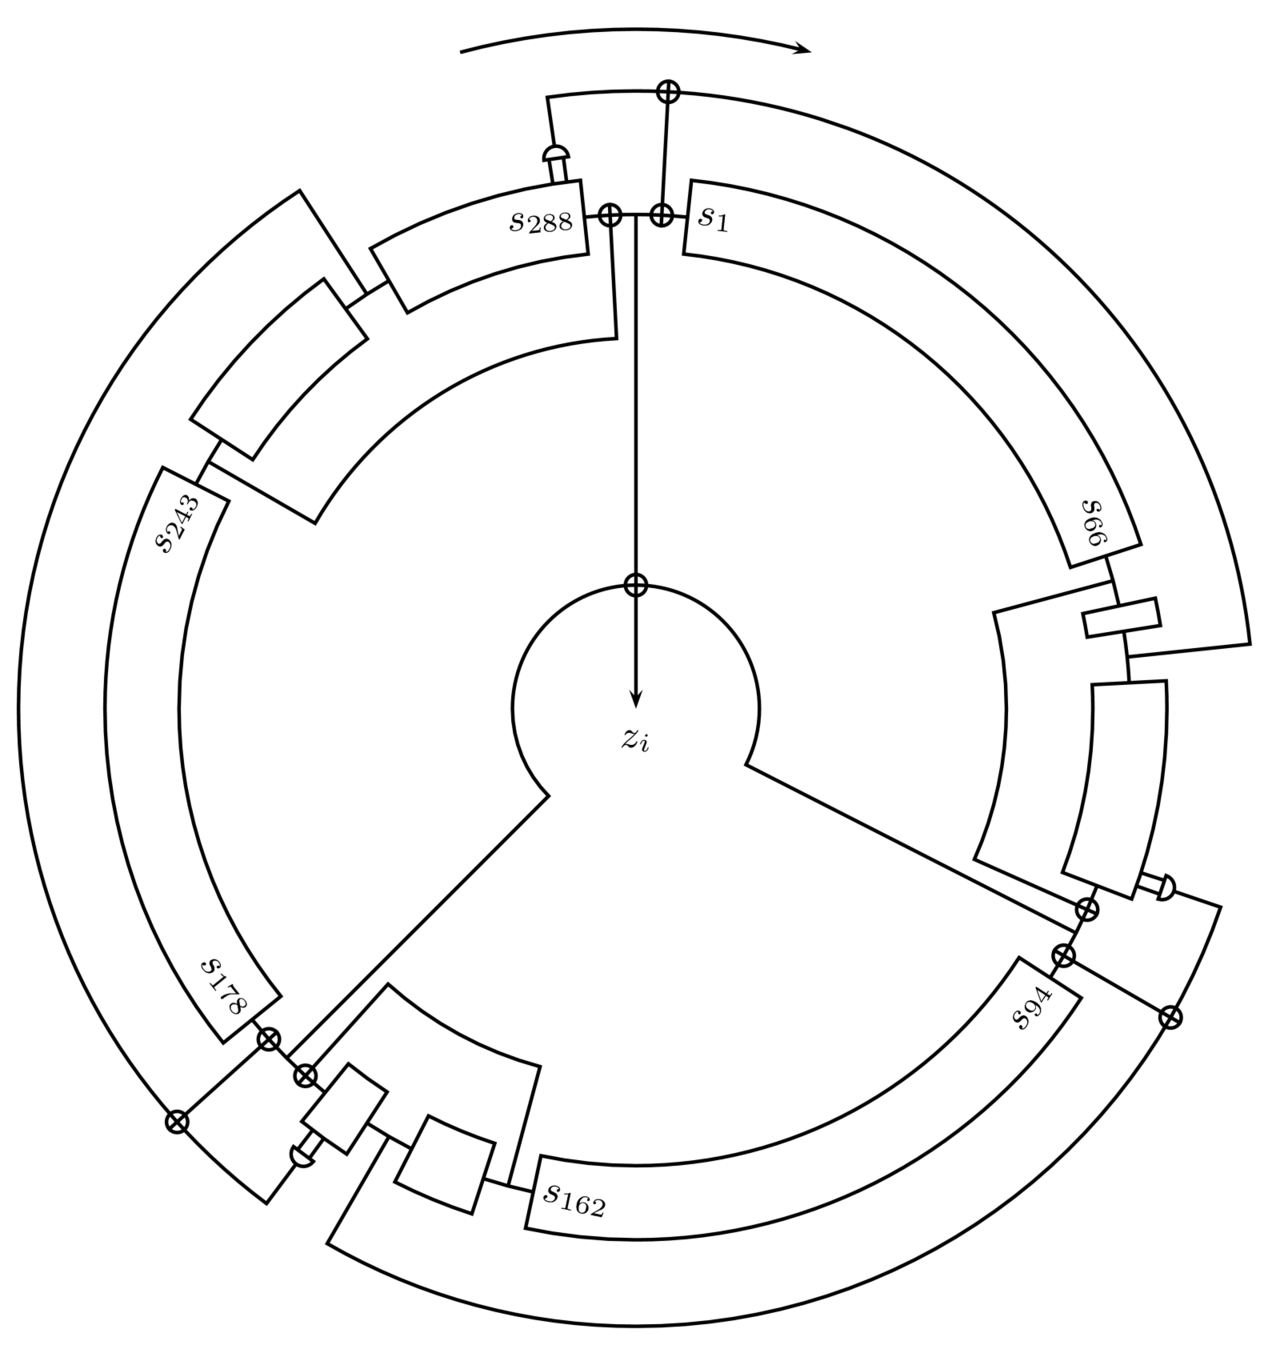
\includegraphics[width=0.9\textwidth]{figures/round.png}\cite{circle}
\end{columns}
\end{frame}

\begin{frame}{Design}
\begin{figure}
\includestandalone[width=0.95\textwidth]{figures/original}
\end{figure}
\end{frame}

\begin{frame}{Key stream generation}
\begin{center}
\begin{minipage}{\textwidth}
\begin{algorithm}[H]
\begin{algorithmic}[1]
\For{$i=1$ to $N$} \Comment{$N\leq 2^{64}$}
\State $t_1 \gets s_{66} + s_{93}$
\State $t_2 \gets s_{162} + s_{177}$
\State $t_3 \gets s_{243} + s_{288}$
\State
\State $z_i \gets t_1 + t_2 + t_3$
\State
\State $t_1 \gets t_1 + s_{91} \cdot s_{92} + s_{171}$
\State $t_2 \gets t_2 + s_{175} \cdot s_{176} + s_{264}$
\State $t_3 \gets t_3 + s_{286} \cdot s_{287} + s_{69}$
\State
\State $(s_1,s_2,\dots,s_{93}) \gets (t_3,s_1,\dots,s_{92})$ \Comment{93 bits}
\State $(s_{94},s_{95},\dots,s_{177}) \gets (t_1,s_{94},\dots,s_{176})$ \Comment{84 bits}
\State $(s_{178},s_{179},\dots,s_{288}) \gets (t_2,s_{178},\dots,s_{287})$ \Comment{111 bits}
\EndFor
\end{algorithmic}
\end{algorithm}
\end{minipage}
\end{center}
\end{frame}

\begin{frame}{Key and IV setup}
\begin{itemize}
\item[$\blacktriangleright$] Run over 4 full cycles
\end{itemize}
\begin{center}
\begin{minipage}{\textwidth}
\begin{algorithm}[H]
\begin{algorithmic}[1]
\State $(s_1,s_2,\dots,s_{93}) \gets (K_1,\dots,K_{80},0,\dots,0)$ \Comment{93 bits}
\State $(s_{94},s_{95},\dots,s_{177}) \gets (IV_1,\dots,IV_{80},0,\dots,0)$ \Comment{84 bits}
\State $(s_{178},s_{179},\dots,s_{288}) \gets (0,\dots,0,1,1,1)$ \Comment{111 bits}
\State
\For{$i=1$ to $4\cdot288$}
\State $t_1 \gets s_{66} + s_{91} \cdot s_{92} + s_{93} + s_{171}$
\State $t_2 \gets s_{162} + s_{175} \cdot s_{176} + s_{177} + s_{264}$
\State $t_3 \gets s_{243} + s_{286} \cdot s_{287} + s_{288}+ s_{69}$
\State
\State $(s_1,s_2,\dots,s_{93}) \gets (t_3,s_1,\dots,s_{92})$ \Comment{93 bits}
\State $(s_{94},s_{95},\dots,s_{177}) \gets (t_1,s_{94},\dots,s_{176})$ \Comment{84 bits}
\State $(s_{178},s_{179},\dots,s_{288}) \gets (t_2,s_{178},\dots,s_{287})$ \Comment{111 bits}
\EndFor
\end{algorithmic}
\end{algorithm}
\end{minipage}
\end{center}
\end{frame}

\section{Attack Scenario}

\begin{frame}{Stuck-at-0 Faults}
\begin{itemize}
\item[$\blacktriangleright$] Injecting stuck-at-0 faults can be done in multiple ways.
\begin{itemize}
\item[$\triangleright$] Binary code modification,
\item[$\triangleright$] FPGA bitsream modification,
\item[$\triangleright$] EM fault injection, 
\item[$\triangleright$] Optical fault injection. 
\end{itemize}
\end{itemize}
\end{frame}

\begin{frame}{Assumptions}
\begin{itemize}[itemsep=0.5cm]
\item[$\blacktriangleright$] Physical access to device; e.g. during shipment.
\item[$\blacktriangleright$] Proprietary protection mechanism, preventing arbitrary code from being run.
\item[$\blacktriangleright$] Code being executed on device is not signed.
\item[$\blacktriangleright$] Lock bits need to protect against read-back are not set.
\item[$\blacktriangleright$] Key is securely stored and cannot be obtained with ease.
\item[$\blacktriangleright$] Key is reused.
\end{itemize}
\end{frame}

\begin{frame}{Procedure}
\begin{itemize}[itemsep=0.5cm]
\item[$\blacktriangleright$] Load fault injected binary onto device.
\item[$\blacktriangleright$] Run fault injected Trivium to obtain $\alpha$ output bits.
\item[$\blacktriangleright$] Cryptanalyse output stream and recover key.
\item[$\blacktriangleright$] Load original binary onto device.
\item[$\blacktriangleright$] Future communications can be deciphered as the key is known.
\end{itemize}
\end{frame}

\section{Fault Injection}

\begin{frame}{Fault Injection}
\begin{figure}
\includestandalone[width=0.95\textwidth]{figures/modified}
\end{figure}
\end{frame}

\begin{frame}{Key stream generation}
\begin{center}
\begin{minipage}{\textwidth}
\begin{algorithm}[H]
\begin{algorithmic}[1]
\For{$i=1$ to $N$} \Comment{$N\leq 2^{64}$}
\State $t_1 \gets s_{66} + s_{93}$
\State $t_2 \gets s_{162} + s_{177}$
\State $t_3 \gets s_{243} + s_{288}$
\State
\State $z_i \gets t_1 + t_2 + t_3$
\State
\State $t_1 \gets t_1 + s_{171}$
\State $t_2 \gets t_2 + s_{264}$
\State $t_3 \gets t_3 + s_{69}$
\State
\State $(s_1,s_2,\dots,s_{93}) \gets (t_3,s_1,\dots,s_{92})$ \Comment{93 bits}
\State $(s_{94},s_{95},\dots,s_{177}) \gets (t_1,s_{94},\dots,s_{176})$ \Comment{84 bits}
\State $(s_{178},s_{179},\dots,s_{288}) \gets (t_2,s_{178},\dots,s_{287})$ \Comment{111 bits}
\EndFor
\end{algorithmic}
\end{algorithm}
\end{minipage}
\end{center}
\end{frame}

\begin{frame}{Key and IV setup}
\begin{itemize}
\item[$\blacktriangleright$] Run over 4 full cycles
\end{itemize}
\begin{center}
\begin{minipage}{\textwidth}
\begin{algorithm}[H]
\begin{algorithmic}[1]
\State $(s_1,s_2,\dots,s_{93}) \gets (K_1,\dots,K_{80},0,\dots,0)$ \Comment{93 bits}
\State $(s_{94},s_{95},\dots,s_{177}) \gets (IV_1,\dots,IV_{80},0,\dots,0)$ \Comment{84 bits}
\State $(s_{178},s_{179},\dots,s_{288}) \gets (0,\dots,0,1,1,1)$ \Comment{111 bits}
\State
\For{$i=1$ to $4\cdot288$}
\State $t_1 \gets s_{66} + s_{93} + s_{171}$
\State $t_2 \gets s_{162} + s_{177} + s_{264}$
\State $t_3 \gets s_{243} + s_{288}+ s_{69}$
\State
\State $(s_1,s_2,\dots,s_{93}) \gets (t_3,s_1,\dots,s_{92})$ \Comment{93 bits}
\State $(s_{94},s_{95},\dots,s_{177}) \gets (t_1,s_{94},\dots,s_{176})$ \Comment{84 bits}
\State $(s_{178},s_{179},\dots,s_{288}) \gets (t_2,s_{178},\dots,s_{287})$ \Comment{111 bits}
\EndFor
\end{algorithmic}
\end{algorithm}
\end{minipage}
\end{center}
\end{frame}

\begin{frame}[fragile]{Binary Code modifications}
\noindent\begin{minipage}{.45\textwidth}
\begin{lstlisting}[style=asm, caption=Original,frame=tlrb]
<_ECRYPT_ivsetup>
and    %esi,%edx    21 f2
and    %esi,%eax    21 f0
and    %eax,%edi    21 c7

<_ECRYPT_process_bytes>
and    %eax,%ebx    21 c3
and    %ebx,%edi    21 df  
and    %eax,%r15d   41 21 c7
<...>

and    %edi,%r9d    41 21 f9
<...>
and    %ecx,%eax    21 c8
and    %eax,%r15d   41 21 c7
<...>
\end{lstlisting}
\end{minipage}\hfill
\begin{minipage}{.45\textwidth}
\begin{lstlisting}[style=asm, caption=Modified,frame=tlrb]
<_ECRYPT_ivsetup>
xor    %esi,%esi    33 f6
xor    %esi,%esi    33 f6
xor    %eax,%eax    33 c0

<_ECRYPT_process_bytes>
xor    %eax,%eax    33 c0
xor    %ebx,%ebx    33 db 
xor    %eax,%eax    33 c0
nop                 90

xor    %edi,%edi    33 ff
nop                 90
xor    %ecx,%ecx    33 c9
xor    %eax,%eax    33 c0
nop                 90
\end{lstlisting}
\end{minipage}
\end{frame}

\section{Cryptanalysis}

\begin{frame}{Key from Initial State}
\begin{itemize}[itemsep=0.5cm]
\item[$\blacktriangleright$] Express initial state as a system of 288 linear equations.
\item[$\blacktriangleright$] Depends on:
\begin{itemize}
\item[$\triangleright$] 80 unknown bits from key
\item[$\triangleright$] 80 known bits from IV
\item[$\triangleright$] 125 bits set to 0
\item[$\triangleright$] 3 bits set to 1
\end{itemize}
\item[$\blacktriangleright$] A system with $k$ unknown variables can be solved using Gaussian elimination in time $k^\alpha$, where $\alpha\leq 2.376$ \cite{gauss}.
\item[$\blacktriangleright$] Finding the solution takes at most $80^{2.376} \leq 33,247$ operations.
\end{itemize}
\end{frame}

\begin{frame}{Initial State from Keystream}
\mbox{\scriptsize
${\displaystyle {\overset {\alpha\times 288{\text{ matrix}}}
{\begin{bmatrix}
a_{1,1}& \dots & a_{1,93} & b_{1,1} & \dots & b_{1,84} & c_{1,1} & \dots & c_{1,111}\\
\vdots &  & \vdots & \vdots &  & \vdots & \vdots &  & \vdots\\
a_{i,1}& \dots & a_{i,93} & b_{i,1} & \dots & b_{i,84} & c_{i,1} & \dots & c_{i,111}\\
\vdots &  & \vdots & \vdots &  & \vdots & \vdots &  & \vdots\\
a_{\alpha,1}& \dots & a_{\alpha,93} & b_{\alpha,1} & \dots & b_{\alpha,84} & c_{\alpha,1} & \dots & c_{\alpha,111}\\
\end{bmatrix}}}
{\overset {288\times 1{\text{ matrix}}}
{\begin{bmatrix}
s_{1} \\
\vdots \\
s_{288} \\
\end{bmatrix}}}
=
{\overset {\alpha\times 1{\text{ matrix}}}
{\begin{bmatrix}
z_{1} \\
\vdots \\
z_{i} \\
\vdots \\
z_{\alpha} \\
\end{bmatrix}}}}
$}

\begin{itemize}[itemsep=0.25cm]
\item[$\triangleright$] $\alpha$ = a time step
\item[$\triangleright$] $a, b, c$ = LFSR 1, 2, 3
\item[$\triangleright$] $s_1,...,s_{288}$ = state variables
\item[$\triangleright$] $z_1,...,z_{\alpha}$ = output bits
\end{itemize}
\end{frame}

\section{Summary}

\begin{frame}{Summary}
\begin{itemize}[itemsep=0.5cm]
\item[$\blacktriangleright$] Stuck-at-0 fault injection attack on binary code.
\item[$\blacktriangleright$] Modify $3 \times 3$ x86 assembly instructions.
\item[$\blacktriangleright$] Injecting stuck-at-0 faults can be done in multiple ways.
\item[$\blacktriangleright$] Reduce the non-linear feedback function to a linear one.
\item[$\blacktriangleright$] The Internal State and Key can be retrieved. 
\end{itemize}
\end{frame}

\begin{frame}{Acknowledgements}
\begin{table}
\centering
\begin{tabular}{l l}
Idea: & Elena Dubrova\\
& \\
Latex Beamer: & \url{github.com/matze/mtheme}\\
& \\
GitHub: & \url{github.com/GaPhil/trivium}
\end{tabular}
\end{table}
\end{frame}

\begin{frame}{Sources}
\bibliography{bibl}
\nocite{*}
\end{frame}

\plain{}{Questions?}

\section{END}

\end{document}